\documentclass[11pt,openany]{book}
\usepackage{blindtext}
\usepackage{tikz,tcolorbox}
\usepackage{xcolor}
\usepackage{amsfonts}
\usepackage{hyperref} 
\usepackage{indentfirst}
\usepackage{graphicx}
\usepackage[normalem]{ulem}
\usepackage [english]{babel}
\usepackage [autostyle, english = american]{csquotes}
\usepackage{appendix}
\usepackage{tabularx}
\usepackage{amsmath,amssymb}
\usepackage{mathtools}
\usepackage{makecell}
\graphicspath{ {./images/} }
\usepackage{enumitem}
\usepackage{soul}
\usepackage{mathtools}
\usepackage{wrapfig}
\usepackage{mathrsfs}
\usepackage{centernot}
\usepackage{amsthm}
\usepackage{listings}
\usepackage{biblatex}
\addbibresource{bibliograph.bib}

\usepackage{pagenote}


\definecolor{codegreen}{rgb}{0,0.6,0}
\definecolor{codegray}{rgb}{0.5,0.5,0.5}
\definecolor{codepurple}{rgb}{0.58,0,0.82}
\definecolor{backcolour}{rgb}{0.95,0.95,0.92}

\lstdefinestyle{mystyle}{
	backgroundcolor=\color{backcolour},   
	commentstyle=\color{codegreen},
	keywordstyle=\color{magenta},
	numberstyle=\tiny\color{codegray},
	stringstyle=\color{codepurple},
	basicstyle=\ttfamily\footnotesize,
	breakatwhitespace=false,         
	breaklines=true,                 
	captionpos=b,                    
	keepspaces=true,                 
	numbers=left,                    
	numbersep=5pt,                  
	showspaces=false,                
	showstringspaces=false,
	showtabs=false,                  
	tabsize=2
}

\lstset{style=mystyle}
%% End notes to be printed as sections at the
%% end of each chapter.
\renewcommand*{\notedivision}{\section*{\notesname}}
\renewcommand*{\pagenotesubhead}[1]{}

\newcommand*{\exercises}{\section*{\exercisename}}
%%%%%%%%%%%%% For customising the endnote markers. Comment these out if you don't want them.
% To prefix each note number with the chapter number
\renewcommand{\thepagenote}{\thechapter-\arabic{pagenote}}

% To have a slightly different formatting for the endnote numbers in the text -- smaller text, sans-serif, square brackets
\renewcommand\notenumintext[1]{\space{\footnotesize\sffamily[FN-#1]}}

% To have a slightly different formatting for the endnote numbers in the notes section. Just the square brackets and sans-serif; normal size.
\renewcommand\notenuminnotes[1]{{\sffamily[FN-#1] }}

% If you want a different name/heading for the end notes
\renewcommand{\notesname}{End Notes}
\newcommand{\exercisename}{Exercises}
%%%%%%%%%%%%% End customisation

\newcommand{\definition}[2]{\begin{tcolorbox}[title=Definition ({#1}),colframe=black]{#2}\end{tcolorbox}
}
%% THIS LINE IS MANDATORY
\makepagenote

\begin{document}
	
	\chapter{Sample - vector calculus}
	
	%in the actual thing, would ideally create a macro to have piecewise smooth reference the definition (in pdf)
	\definition{Line Integral - scalar}{
		Let $U \subset \mathbb{R}^n$, $\gamma \subset U$ be a piecewise smooth curve, and $f: U \to \mathbb{R}$. The \textbf{line integral of $f$ along $\gamma$} is defined as
		\[
		\int_\gamma \ f \ ds \ = \ \int_a^b f(r(t)) \ |r'(t)| \ dt
		\]
		where $r : [a,b] \to \gamma$ is any parameterization of $\gamma$.
	}
	\definition{Line Integral - vector}{
		Let $U \subset \mathbb{R}^n$, $\gamma \subset U$ be a piecewise smooth curve, and $f: U \to \mathbb{R}^n$. The \textbf{line integral of $f$ along $\gamma$} is defined as
		\[
		\int_\gamma \ f \ ds \ = \ \int_a^b f(r(t)) \cdot r'(t)  \ dt
		\]
		where $r : [a,b] \to \gamma$ is any parameterization of $\gamma$.
	}
	\section*{Geometric intuition}
	%todo - plot in python
	For a visualization, let's plot a 2D function (so visualizing the graph in 3D) in Python. We want to integrate the function $f(x,y)=\sin(x+y)$ along the semi-unit-circle in the top half plane, oriented counter-clockwise. This can be parametrized by $r(t) = (\cos(t), \sin(t))$ for $t\in [0,\pi / 2]$. 
	\begin{lstlisting}[language=Python]
		import matplotlib.pyplot as plt
		import numpy as np
		#create figure
		ax = plt.figure().add_subplot(projection='3d')
		
		#plot sin(x+y)
		X,Y=np.meshgrid(np.linspace(-1,1,40), np.linspace(-1,1,40))
		Z=np.sin(X+Y)
		surface=ax.plot_surface(X, Y, Z, alpha=0.5,
		label='graph surface')
		ax.set_xlabel('x')
		ax.set_ylabel('y')
		ax.set_zlabel('sin(x+y)')
		
		#plot the curve and the cross section to integrate
		curve=np.linspace(0,np.pi,40)
		plot_curve=ax.plot(np.cos(curve), np.sin(curve), 0,
		label='cross section to integrate')
		curvevalues=np.sin(np.cos(curve)+np.sin(curve))
		curveonsurface=ax.bar3d(np.cos(curve),np.sin(curve),0,
		dx=0.01, dy=0.01, dz=curvevalues, alpha=0.5,
		color='orange')
		
		plt.legend()
		plt.show()
	\end{lstlisting}
	\begin{wrapfigure}{r}{0.75\textwidth} 
		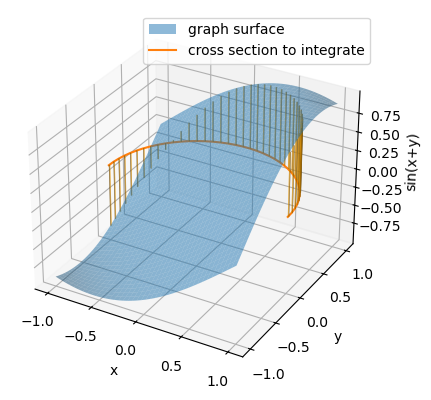
\includegraphics[width=0.75\textwidth]{sin.png}
	\end{wrapfigure}
	
	
\end{document}